\documentclass[a4paper,12pt]{article}
\usepackage[T1,T2A]{fontenc}
\usepackage[utf8]{inputenc}
\usepackage[english,ukrainian]{babel}

\usepackage{ upgreek }
\usepackage{amsmath}

\usepackage{graphicx}
\graphicspath{{../pictures/}}
\DeclareGraphicsExtensions{.pdf,.png,.jpg}

\usepackage{hyperref}
\hypersetup{colorlinks = true}
\usepackage{geometry} % Меняем поля страницы
\geometry{left=2cm}% левое поле
\geometry{right=1.5cm}% правое поле
\geometry{top=1cm}% верхнее поле
\geometry{bottom=2cm}% нижнее поле



\begin{document}
	
\begin{titlepage}
	\vspace*{6cm}
	\begin{center}
		
		\large
		\textbf{Звіт}\\
		\textbf{до лабораторної роботи №2:}\\
		\textbf{<<Застосування
			методу дискретних особливостей для\\
			моделювання аеродинамічних процесів>>}
		
	\end{center}
	
	\vspace{8cm}
	\begin{flushright}
		студента 1-го курсу магістратури\\
		факультету комп'ютерних наук та кібернетики\\
		Кравця Олексія
	\end{flushright}
	
\end{titlepage}

\newpage
	
\section{Постановка задачі}
	
	
	Дано контур $L_d$, що знаходиться в області $D$, з течією на нескінченості $V_{\infty} = (u_{\infty}(t), v_{\infty}(t))$. Позначимо через $L_v$ вільну границю. Також вважаємо, що течія безвихорова, тобто $\exists \varphi = \varphi(x,y,t) : \vec{V} = \nabla \varphi$. Потенціал $\varphi$ в області $D$ задовольняє рівняння Лапласа: $\Updelta \varphi =0$.
	
	Крім того на контурі $L_d$ виконується умова непроникності:
	\[
		\left( \nabla \varphi \cdot \vec{n} \right)|_{L_d} = 0,
	\]
	де $\vec{n}$ -- нормаль до поверхні $L_d$.
	
	На вихровому контурі $L_v$ виконуються такі умови:
	\begin{align}
		\left( \frac{\partial \varphi}{\partial \vec{n}} \right)^+ &= \left( \frac{\partial \varphi}{\partial \vec{n}} \right)^- \quad \text{на } L_v \nonumber \\
		p^+ &= p^- \quad \text{на } L_v \nonumber
	\end{align}
	
	Також вважаємо, що $\lim_{|r| \rightarrow \infty} \nabla \varphi = \vec{V}_{\infty}$, тобто із нескінченності набігає потік сталої швидкості. Також вважаємо, що швидкість скінченна $|\nabla \varphi| < \infty$ на гострих кутах $L$.
	
	Інтеграл Коші-Лагранжа:
	\[
	\frac{\nabla \varphi}{\nabla t} + \frac{1}{2}\left( \nabla \varphi \right)^2 + \frac{p}{\rho} = \frac{p_{\infty}}{\rho} + \frac{1}{2} V_{\infty}^2 + \frac{\nabla \varphi_{\infty}}{\nabla t}
	\]
	Інтегральне представлення аналітичного розв'язку:
	\begin{align}
		\Phi(z,t) &= \varphi + i\xi = \vec{V}_\infty z + \frac{1}{2 \pi i} \int_{L_d(t)} f(w,t) \ln{(z - w)}dw + \frac{1}{2 \pi i} \int_{L_v(t)} f(w,t) \ln{(z - w)}dw + const \nonumber \\
		\vec{V}(z,t) &= u- iv = \frac{\nabla \Phi(z,t)}{\nabla z} = \vec{V}_\infty + \frac{1}{2 \pi i} \int_{L_d(t)} \frac{f(w,t)}{z - w} dw + \frac{1}{2 \pi i} \int_{L_v(t)} \frac{f(w,t)}{z - w} dw \nonumber
	\end{align}
\section{Моделювання кінематики}

	Необхідно дискретизувати контур, розіб'ємо його на $M$ точок $(x_{0j}, y_0j), j = \overbrace{1,M}$. Тепер знайдемо точки колокації:
	\begin{eqnarray}
		x_k = \frac{x_{0k} + x_{0, k+1}}{2} \nonumber \\
		y_k = \frac{y_{0k} + y_{0, k+1}}{2} \nonumber
	\end{eqnarray}
	
	Також проведемо нормалі в точках колокацій:
	
	\begin{align} 
		\overrightarrow{n_k} (x_k, y_k) = (n_{xk}, n_{yk}),\quad  k = \overline{1, M-1} \nonumber \\
		n_{xk} = \frac{-(y_{0,k+1} - y_{0k})}{\sqrt{(x_{0, k+1} -  x_{0k})^2 + (y_{0,k+1} - y_{0k})^2}} \nonumber \\
		n_{yk} = \frac{x_{0, k+1} -  x_{0k}}{\sqrt{(x_{0, k+1} -  x_{0k})^2 + (y_{0,k+1} - y_{0k})^2}} \nonumber
	\end{align}
	
	\begin{figure}[ht]
		\begin{center}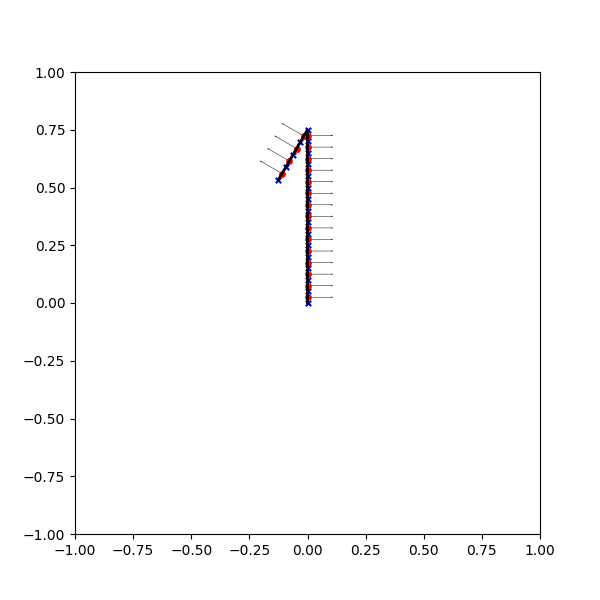
\includegraphics[scale=0.5]{obstacle_1_for_report} \end{center}
		\caption{Вигляд контуру}
		\label{fig:obstale_1_for_report}
	\end{figure}
	
	На рисунку ($\ref{fig:obstale_1_for_report}$) бачимо вигляд контуру. Синіми хрестами позначені точки дискретних особливостей, з червоних точок колокацій виходять нормалі. Напрям нормалей залежить від напрямку обходу контуру. В цьому випадку, ми починаємо рухатися від лівого верхнього кінця і закінчуємо у правому нижньому.

	Тепер розв'яжемо задачу чисельно. Вважаємо, що модуль швидкості $|\vec{V}_\infty| = 1$, тобто $V_\infty = (\cos{\alpha}, \sin{\alpha})$. Для обчислення потенціалу і швидкості в момент часу $t = t_{n+1}$ будемо використовувати наступні формули:
	\newpage

	\begin{align}
		\varphi(x,y,t_{n+1}) &= (x \cos \alpha + y \sin \alpha) + \sum\limits_{j=1}^{M} \frac{\Gamma_j(t_{n+1})}{2 \pi} Arctg \left(\frac{y - y_{0j}}{x - x_{0j}}\right)  \nonumber \\ &+\sum_p \sum\limits_{i=1}^{n+1} \frac{\gamma_{i}^{p}}{2 \pi} Arctg \left( \frac{ y - y_{i}^{p}(t_{n+1}) }{ x - x_{i}^{p} (t_{n+1}) }\right) \nonumber	
	\end{align}
	
	\begin{align}
		\vec{V}(x,y,t_{n+1}) &= (\cos \alpha, \sin \alpha) + \sum_{j=1}^{M} \Gamma_{j}(t_{n+1}) \vec{V}(x,y,x_{0j}, y_{0j}) \nonumber \\ &+\sum_p \sum_{i=1}^{n+1} \gamma_{i}^{p} \vec{V}(x,y,x_{i}^{p}(t_{n+1}), y_{i}^{p}(t_{n+1})) \nonumber
	\end{align}

	Перед тим, як почати розв'язувати ці рівняння, введемо декілька величин.
	\begin{equation*}
		R_{0i} = 
		\begin{cases}
			\sqrt{ (x - x_{0i})^2 + (y - y_{0i})^2 }, &\sqrt{ (x - x_{0i})^2 + (y - y_{0i})^2 } > \delta
			\\
			\qquad \delta, &\sqrt{ (x - x_{0i})^2 + (y - y_{0i})^2 } \le \delta
		\end{cases}
	\end{equation*}
	
	\begin{equation*}
		\vec{V}(x,y,x_{0i}, y_{0i}) =
		\begin{cases}
			u(x,y,x_{0i}, y_{0i}) = \frac{1}{2 \pi} \frac{y_{0i} - y}{R_{0i}^2}
			\\
			v(x,y,x_{0i}, y_{0i}) = \frac{1}{2 \pi} \frac{x - x_{0i} }{R_{0i}^2}
		\end{cases}
	\end{equation*}
	
	Для того, щоб знайти коефіцієнти $\Gamma_{j}$ необхідно розв'язати систему лінійних алгебраїчних рівнянь.
	
	\begin{equation*}
		\begin{cases}
			\sum_{j=1}^{M} \Gamma_{j}(t_{n+1})\left( \vec{V}(x_k,y_k, x_{0j}, y_{0j}) \cdot \vec{n}(x_k,y_k) \right) = - \left[ \left(  \vec{V}_{\infty} \cdot \vec{n}(x_k, y_k) \right) \right.
			\\
			+ \left. \sum_p \sum_{i=1}^{n+1} \gamma_{i}^{p} \left( \vec{V}(x_k,y_k,x_{i}^{p}(t_{n+1}), y_{i}^{p}(t_{n+1})) \cdot \vec{n}(x_k, y_k) \right)\right], k = \overline{1,M-1}
			\\
			\sum_{j=1}^{M} \Gamma_{j}(t_{n+1}) = - \sum_p \sum_{i=1}^{n+1} \gamma_{i}^{p}
		\end{cases}
	\end{equation*}
	
	Одночасно з цим проходить оновлення точок вихорової границі. Для цього використовуємо метод Ейлера. Тобто $\forall p, i = \overline{1,n}$:
	\begin{equation*}
		\begin{cases}
			x_{i}^{p}(t_{n+1}) = x_{i}^{p}(t_n) + u(x_{i}^{p}(t_n), y_{i}^{p}(t_n), t_n)\tau_n
			\\
			y_{i}^{p}(t_{n+1}) = y_{i}^{p}(t_n) + v(x_{i}^{p}(t_n), y_{i}^{p}(t_n), t_n)\tau_n
		\end{cases}
	\end{equation*}
	де $$\tau_n = \frac{\min_{k} \delta_k}{\max_{D}(|V|)}.$$

	На кожному кроці з кінцевих та кутових точок перешкоди вилітають нові вихорові точки. При цьому, вони мають такі властивості:
	\[
		\forall p: \gamma_{n+1}^{p} = \Gamma_p(t_n);
	\]
	\begin{equation*}
		\begin{cases}
			x_{n+1}^{p}(t_{n+1}) = x_{0p}(t_n) + u(x_{0p}(t_n), y_{0p}(t_n), t_n)\tau_n
			\\
			y_{n+1}^{p}(t_{n+1}) = y_{0p}(t_n) + v(x_{0p}(t_n), y_{0p}(t_n), t_n)\tau_n
		\end{cases}
	\end{equation*}
	
	\subsection{Забезпечення непроникності контуру $L_d$.}
	
		Для забезпечення непроникності контуру необхідно накласти деякі умови. Відстань між двома точками дискретних особливостей повинна бути меньше за $2\delta$, де $\delta$ -- константа, що використовується для розрахунку $\tau$. Це дає нам змогу відслідковувати ті вихорові точки, що наблизилися до границі.
		
		Нехай маємо точку дискретної особливості $z_0 = (x_0, y_0)$, до якої наблизилася точка вихорової границі $z_1(t_{n+1}) = (x_i(t_{n+1}), y_i(t_{n+1}))$ на відстань менше $2 \delta$.
		
		Необхідно зрозуміти з якої сторони контуру наблизилася вихорова точка. Тому візьмемо точку $z_1(t_{n})$ -- точку де була точка $z_1(t_n+1)$ на минулому кроці, та обрахуємо $\lambda = sign \left( (\vec{n_0}, z1(t_n) - z_0) \right)$, де $\vec{n_0}$-- нормаль в точці $z_0$
		
		 Тепер можна обрахувати коефіцієнт $k = \lambda|z0 - z1|$. Отже змінимо точку $z_1(t_{n+1}) = z_1(t_n) + k\vec{n_0}$.
		
\section{Результати}
	Щоб переглянути анімації перейдіть по \href{https://github.com/AlKravets/nonclassical-optimization-lab2}{ссилці}.

\section{Висновок}
	Було змодельовано задачу обтікання заданого непроникного контура. Для розв'язання даної задачі було використано метод дискретних особливостей. Були отримані анімовані результати. Потрібно зазначити, що реалізація непроникності контуру має помилки, але в модельних задачах вони не впливають на глобальний результат.

\end{document}